\documentclass[a4paper,12pt]{article} 

%paquetes
\usepackage{graphicx}
\usepackage[spanish]{babel} 
\usepackage[utf8]{inputenc}
\usepackage{textcomp}
\usepackage{amssymb}
\usepackage{amsmath}
\usepackage{float}
\usepackage{subfig}
\usepackage{listings}
\lstset
{ %Formatting for code in appendix
    language=Matlab,
    basicstyle=\footnotesize,
    numbers=left,
    stepnumber=1,
    showstringspaces=false,
    tabsize=4,
    breaklines=true,
    breakatwhitespace=false,
}

%caracteristicas de paginas
\pdfpagewidth 8.5in
\pdfpageheight 11in
\setlength\oddsidemargin{-0,21in}
\setlength\evensidemargin{-0,21in}
\setlength\topmargin{-2cm}
\setlength\textwidth{7in}
\setlength\textheight{9in}
\setlength\parskip{0.1in}

%%%%%%%%%%%%%%%%%%%%%%%%%%%%%%%%%%%%%%%%%%%%%%%%%%%%%%%%%%%%%

\begin{document} 

\title{Simulaci\'on del modelo de Ising en 2D \\
\large Pr\'actica computacional - F\'isica Te\'orica 3 ($1^{er}$ cuat. 2018) - Clase P. Minnini}
\author{Ignacio Poggi - L.U: 567/07 - ignaciop.3@gmail.com}
\maketitle

%\tableofcontents  %lo ponemos para trabajo largos que necesiten indice
\section{Notas}

Se tomaron las siguientes constantes a lo largo del trabajo:

\begin{itemize}
\item $k_{B}$ = 1
\item $J$ = 1
\item $B$ = 0
\end{itemize}

En el Ap\'endice se transcribe el c\'odigo fuente utilizado en lenguaje Matlab.

\section{Ejercicio: Tiempo de equilibraci\'on}

Para obtener el numero de iteraciones necesarias para que la energ\'ia y la magnetizaci\'on alcancen un equilibro, se eligieron tres tama\~nos de la red posibles: $L$ = 16, $L$ = 32 y $L$ = 64.
A su vez, para cada $L$ se analizaron los siguientes valores de temperatura: $T$ = 1.8 ($T < T_{c}$), $T$ = 2.27 ($T = T_{c}$) y $T$ = 3 ($T > T_{c}$).

Se fijo una cota superior razonable de $n$ = 10000 iteraciones totales; de esta manera se puede cubrir una rango lo suficiente grande para permitir que cada sistema termalice y luego alcance el equilibrio; sin esperar tiempos muy largos de ejecuci\'on del c\'odigo.

\subsection{Resultados}

Se encontr\'o que para $T$ = 1.8, el numero de iteraciones para que la energ\'ia y la magnetizaci\'on de cada sistema llegue al equilibro var\'ia con el tama\~no de la red; es decir a mayor $L$, m\'as iteraciones se necesitan para que el sistema alcance el equilibro en los par\'ametros observados.


\begin{figure}[H]
\begin{center}
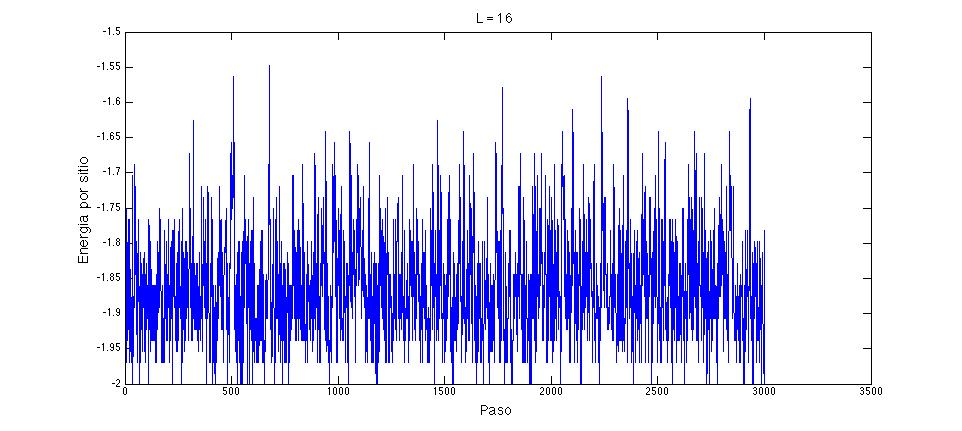
\includegraphics[height=8cm]{../graficos/En_L16_T18.jpg}
\caption[width=5cm]{Convergencia de la energ\'ia por sitio para $L$ = 16 y $T$ = 1.8.}
\end{center}
\end{figure}

\begin{figure}[H]
\begin{center}
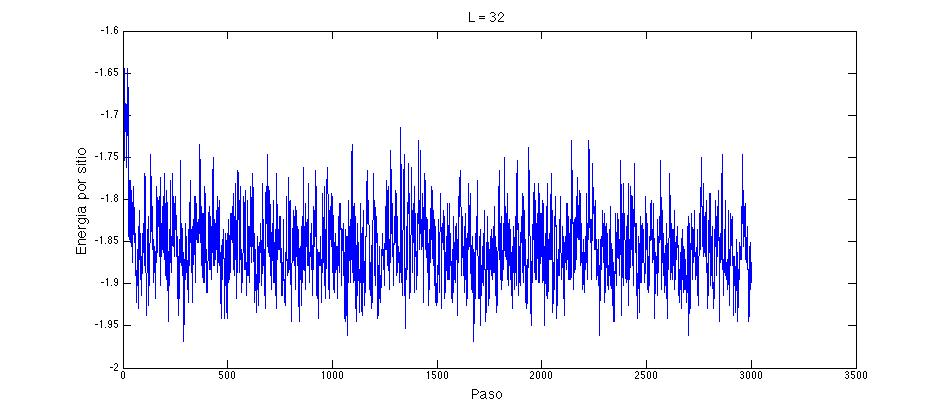
\includegraphics[height=8cm]{../graficos/En_L32_T18.jpg}
\caption[width=5cm]{Convergencia de la energ\'ia por sitio para $L$ = 32 y $T$ = 1.8.}
\end{center}
\end{figure}

\begin{figure}[H]
\begin{center}
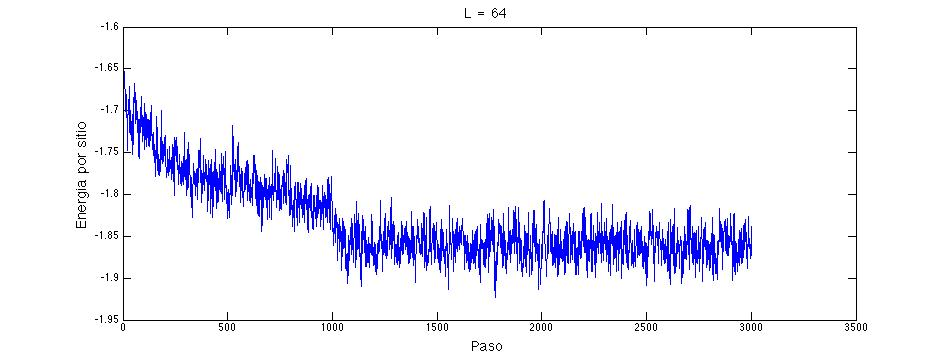
\includegraphics[height=8cm]{../graficos/En_L64_T18.jpg}
\caption[width=5cm]{Convergencia de la energ\'ia por sitio para $L$ = 64 y $T$ = 1.8.}
\end{center}
\end{figure}

\begin{figure}[H]
\begin{center}
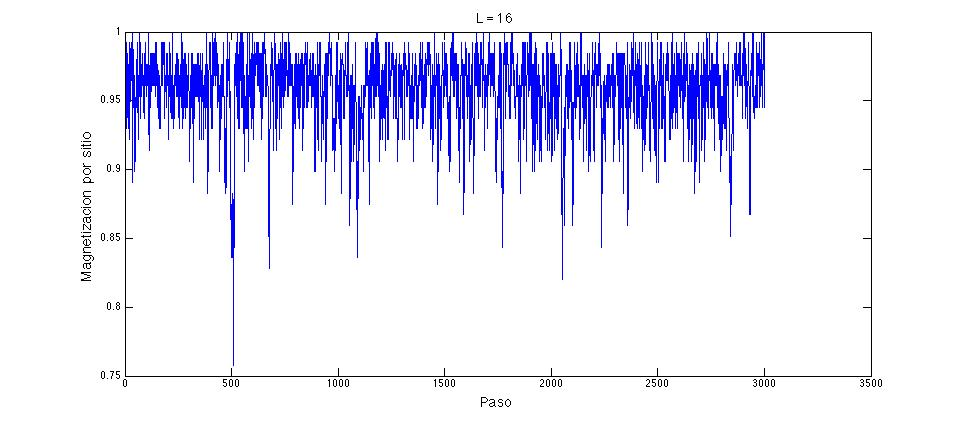
\includegraphics[height=8cm]{../graficos/Mag_L16_T18.jpg}
\caption[width=5cm]{Convergencia de la magnetizaci\'on por sitio para $L$ = 16 y $T$ = 1.8.}
\end{center}
\end{figure}

\begin{figure}[H]
\begin{center}
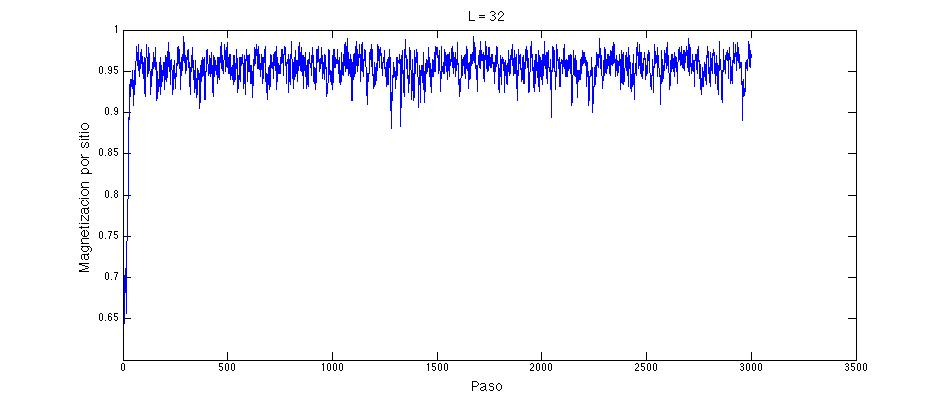
\includegraphics[height=8cm]{../graficos/Mag_L32_T18.jpg}
\caption[width=5cm]{Convergencia de la magnetizaci\'on por sitio para $L$ = 32 y $T$ = 1.8.}
\end{center}
\end{figure}

\begin{figure}[H]
\begin{center}
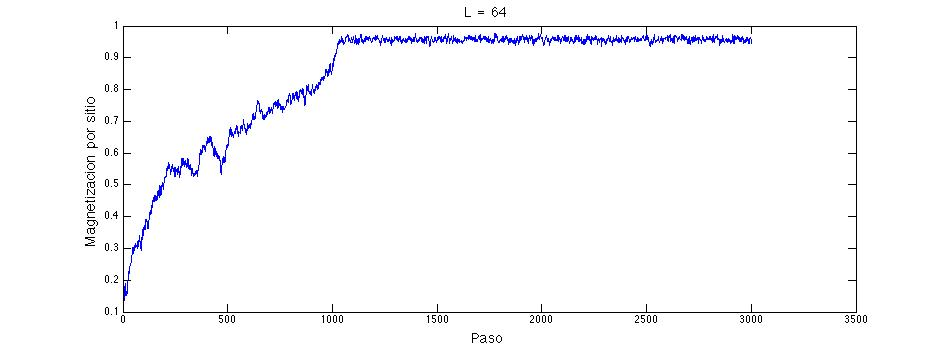
\includegraphics[height=8cm]{../graficos/Mag_L64_T18.jpg}
\caption[width=5cm]{Convergencia de la magnetizaci\'on por sitio para $L$ = 64 y $T$ = 1.8.}
\end{center}
\end{figure}


En las siguientes tablas, se muestran los resultados obtenidos de $n$ para la energ\'ia y la magnetizaci\'on por sitio en cada caso:

\begin{table}
	\centering
    \begin{tabular}{ | l | l | l | l | l |p{5cm} |}
    \hline
    $L = 16$ & $L = 32$ & $L = 64$\\ \hline
    $n \approx$ 250 & $n \approx$ 500 & $n \approx$ 1250  \\ \hline
        
    \end{tabular}
    \caption{Cantidad de iteraciones $n$ para alcanzar el equilibrio en $e$ y $m$ a $T$ = 2.27 = $T_{c}$, para cada valor de $L$.}
    \label{table:1}
\end{table}


Cabe aclarar que, si bien en algunos casos (por ejemplo para $L$ = 64), el $n$ observado puede ser menor al informado en la tabla, se escogi\'o un enfoque m\'as conservativo; esto significa que no se tabul\'o un $n$ justo en la zona de termalizaci\'on-equilibrio; sino que se eligi\'o un valor posterior.

En el caso $T$ = 2.27 = $T_{c}$, se pudo observar que la energ\'ia oscila en torno a un mismo valor medio ($e \approx -1.4$) casi inmediatamente al inicio de la ejecuci\'on del c\'odigo; adem\'as de que dicho valor es m\'as estable a medida que $L$ es mayor, como se observa en las siguientes figuras:

\begin{figure}[H]
\begin{center}
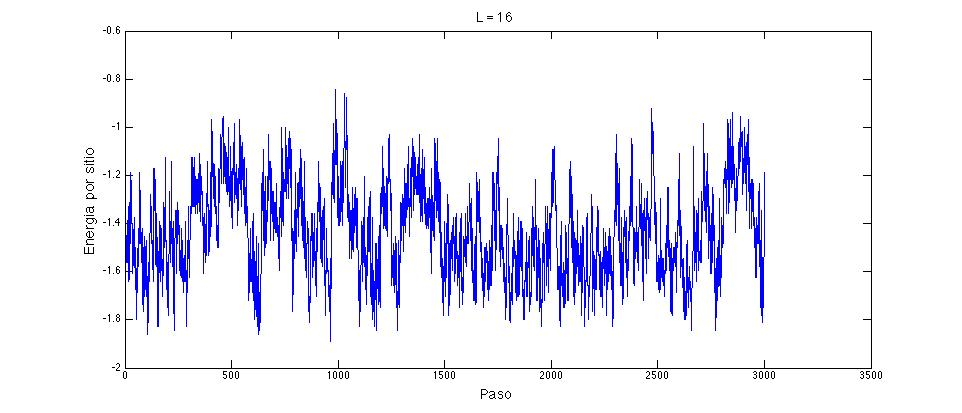
\includegraphics[height=8cm]{../graficos/En_L16_T227.jpg}
\caption[width=5cm]{Convergencia de la energ\'ia por sitio para $L$ = 16 y $T$ = 2.27.}
\end{center}
\end{figure}

\begin{figure}[H]
\begin{center}
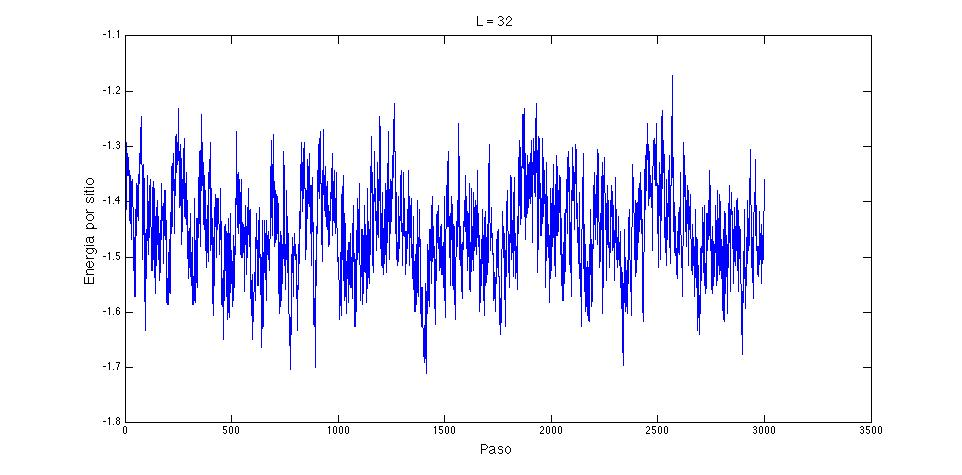
\includegraphics[height=8cm]{../graficos/En_L32_T227.jpg}
\caption[width=5cm]{Convergencia de la energ\'ia por sitio para $L$ = 32 y $T$ = 2.27.}
\end{center}
\end{figure}

\begin{figure}[H]
\begin{center}
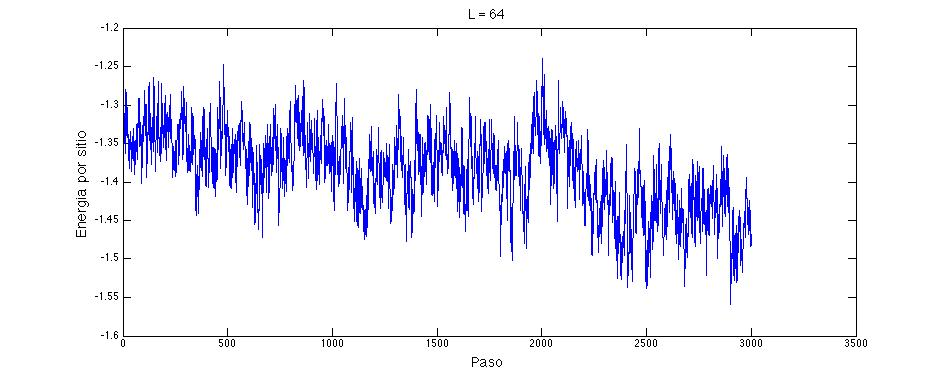
\includegraphics[height=8cm]{../graficos/En_L64_T227.jpg}
\caption[width=5cm]{Convergencia de la energ\'ia por sitio para $L$ = 64 y $T$ = 2.27.}
\end{center}
\end{figure}


Como es de esperar en este caso, el valor absoluto de la magnetizaci\'on oscila entre 0 y -1 de manera muy brusca para cada valor de $L$ estudiado, por lo tanto no se puede decir que dicho observable converja para alg\'un valor de $n$; pero s\'i se puede asegurar que este comportamiento oscilatorio se mantiene durante toda la ejecuci\'on del programa con el valor de $T$ considerado en este caso; lo que es consistente con la teor\'ia.

\begin{figure}[H]
\begin{center}
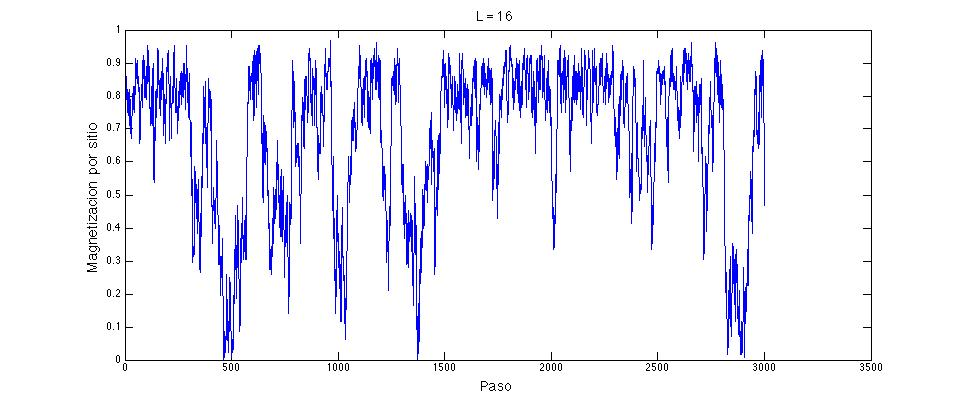
\includegraphics[height=8cm]{../graficos/Mag_L16_T227.jpg}
\caption[width=5cm]{Convergencia de la magnetizaci\'on por sitio para $L$ = 16 y $T$ = 2.27.}
\end{center}
\end{figure}

\begin{figure}[H]
\begin{center}
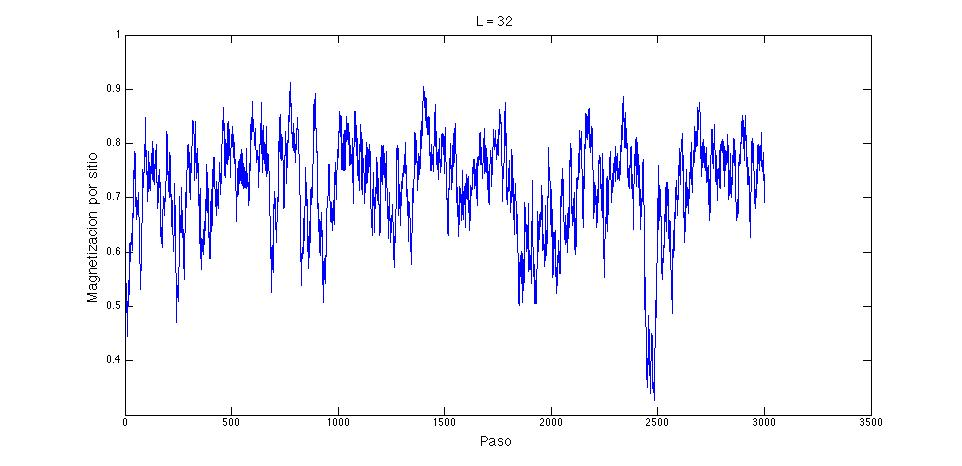
\includegraphics[height=8cm]{../graficos/Mag_L32_T227.jpg}
\caption[width=5cm]{Convergencia de la magnetizaci\'on por sitio para $L$ = 32 y $T$ = 2.27.}
\end{center}
\end{figure}

\begin{figure}[H]
\begin{center}
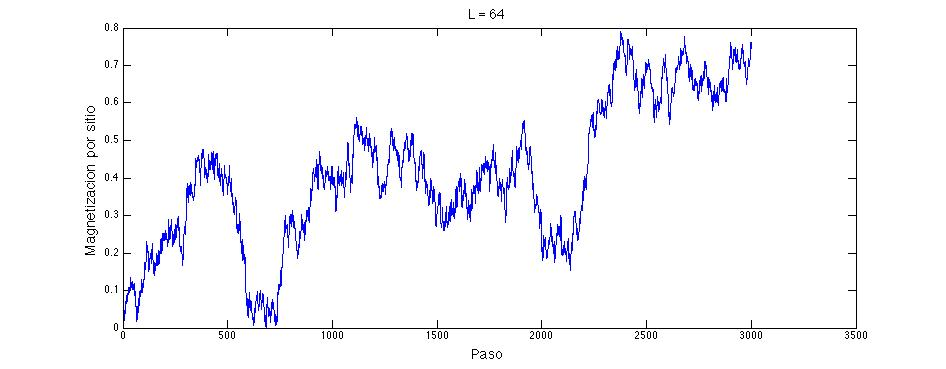
\includegraphics[height=8cm]{../graficos/Mag_L64_T227.jpg}
\caption[width=5cm]{Convergencia de la magnetizaci\'on por sitio para $L$ = 64 y $T$ = 2.27.}
\end{center}
\end{figure}

Por \'ultimo, para $T = 3 > T_{c}$, tanto la energ\'ia como la magnetizaci\'on de cada $L$ converge aproximadamente a $-0.8$ y 0 respectivamente para un $n$ muy peque\~no: se podr\'ia tomar uno casi inmediato al comienzo de la ejecuci\'on del programa. En este caso, los gr\'aficos para $e$ y $m$ son similares para los tres valores de $L$. Como ejemplo, se muestran los mismos para $L$ = 64:

\begin{figure}[H]
\begin{center}
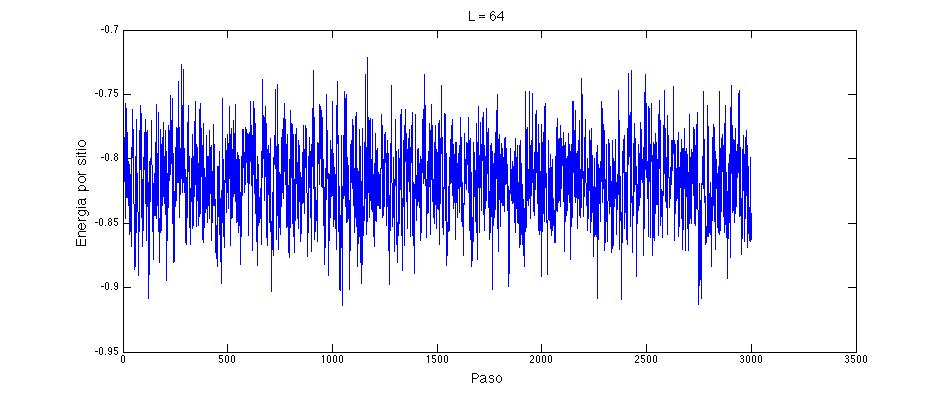
\includegraphics[height=8cm]{../graficos/En_L64_T3.jpg}
\caption[width=5cm]{Convergencia de la energ\'ia por sitio para $L$ = 64 y $T$ = 3.}
\end{center}
\end{figure}

\begin{figure}[H]
\begin{center}
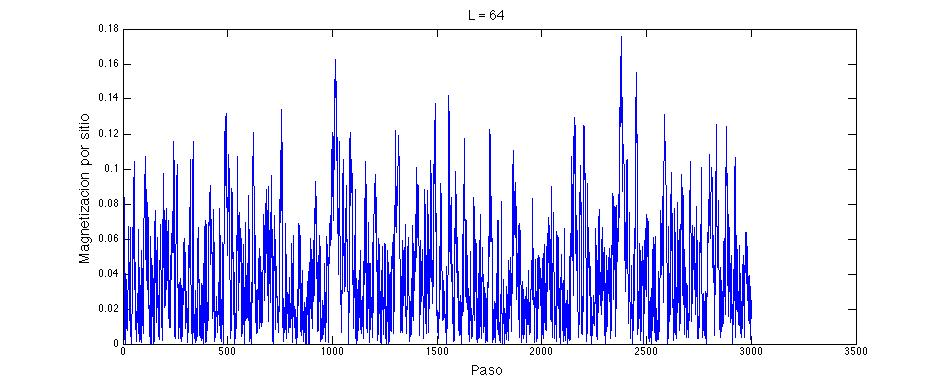
\includegraphics[height=8cm]{../graficos/Mag_L64_T3.jpg}
\caption[width=5cm]{Convergencia de la magnetizaci\'on por sitio para $L$ = 64 y $T$ = 3.}
\end{center}
\end{figure}


\subsection{Conclusi\'on}

Para este ejercicio, el r\'egimen mas interesante a estudiar fue el caso $T < T_{c}$, donde se obtuvo que a mayor $L$, son necesarias m\'as cantidad de iteraciones para que el sistema alcance el equilibro en los observables medidos. Para $T > T_{c}$, $n$ fue despreciable para llegar a dichos equilibrios; en el caso $T = T_{c}$, no tiene sentido hablar de convergencia en la magnetizaci\'on por la naturaleza oscilatoria del mismo en este r\'egimen; pero para la energ\'ia el comportamiento es similar al caso $T > T_{c}$, por lo tanto se puede concluir que, en lineas generales, la convergencia de los valores medidos de los observables depende de la temperatura, pero a temperaturas bajas es necesario considerar tambi\'en el tama\~no de la red.


\section{Ejercicio: Energ\'ia y magnetizaci\'on en funci\'on de la temperatura}

En este ejercicio se tuvieron presentes los resultados del anterior en lo referido a la cantidad de iteraciones necesarias para que el sistema llegue al equilibrio. Por esto, para calcular la energ\'ia y magnetizaci\'on media ($<e> y <m>$ respectivamente), se eligi\'o un $n$ = 3000 para valores de $T$ entre 0 y 10; con pasos de 0.2; debido a que es un numero razonable de iteraciones para que el sistema termalice, llegue al equilibrio y un tiempo extra poder tomar valores medios significativos.

\subsection{Resultados}

A continuaci\'on, se muestran los resultados adquiridos para $L$ = 16:

\begin{figure}[H]
\begin{center}
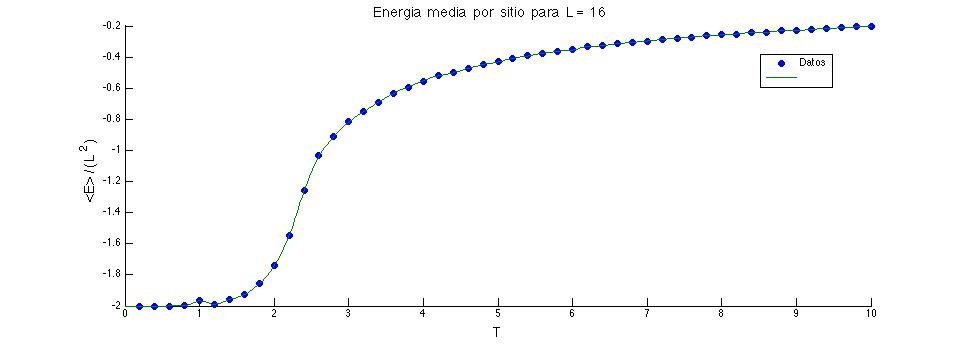
\includegraphics[height=8cm]{../graficos/Emean_L16.jpg}
\caption[width=5cm]{Energ\'ia media por sitio para $L$ = 16.}
\end{center}
\end{figure}

Se puede observar que, para $T \rightarrow 0$, la energ\'ia media tiende a $-2$; de acuerdo con la teor\'ia (tomando $J$ = 1). En un entorno de Tc, se da un salto hacia un valor mayor; esto se corresponde a la transici\'on de fase, que se observar\'a m\'as adelante como una discontinuidad en los gr\'aficos correspondientes al $C_{v}$. La energ\'ia tiende a estabilizarse alrededor de $-0.2$ cuando $T >> T_{c}$.

\begin{figure}[H]
\begin{center}
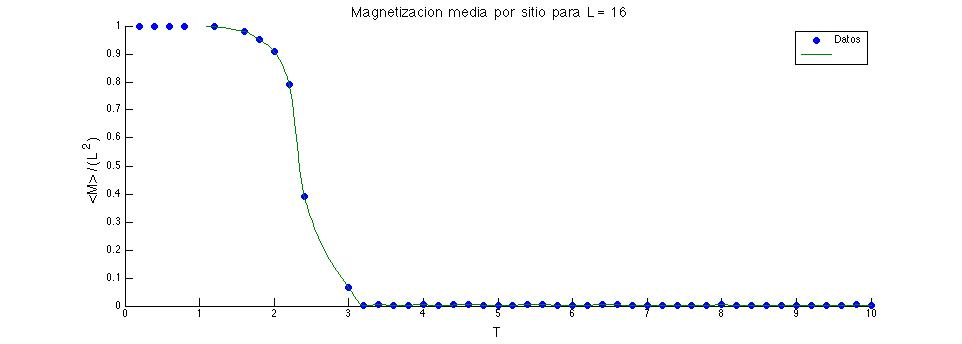
\includegraphics[height=8cm]{../graficos/Mmean_L16.jpg}
\caption[width=5cm]{Magnetizaci\'on media por sitio para $L$ = 16.}
\end{center}
\end{figure}

Ac\'a se puede ver que la magnetizaci\'on mantiene un valor medio estable en 1 para valores de $T < T_{c}$; esto puede interpretarse como que todos los spines tienen el mismo valor. Al llegar a la temperatura cr\'itica se observa un salto (discontinuidad) en el valor de $<m>$ correspondiente al cambio de fase, convergiendo r\'apidamente a 0 para temperaturas mayores a $T_{c}$, lo que indica la p\'erdida de magnetizaci\'on de la muestra.


Para calcular el calor espec\'ifico y la susceptibilidad magn\'etica, se utilizaron las f\'ormulas dadas por el enunciado, relacion\'andolas de la siguiente manera:

\begin{itemize}
\item $C_{v} = \frac{\sigma_{E}^{2}}{T^2}$ 
\item $\chi_{m} = \frac{\sigma_{M}^{2}}{T}$ 
\end{itemize}

Los resultados para estos observables fueron los siguientes:

\begin{figure}[H]
\begin{center}
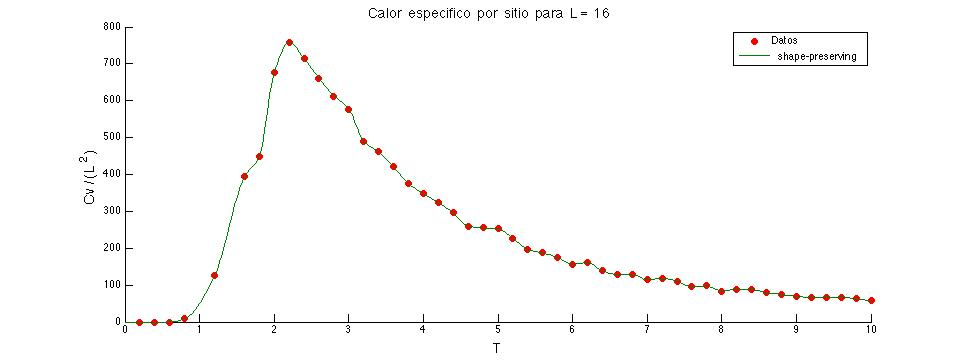
\includegraphics[height=8cm]{../graficos/Cv_L16.jpg}
\caption[width=5cm]{Calor espec\'ifico por sitio para $L$ = 16.}
\end{center}
\end{figure}

\begin{figure}[H]
\begin{center}
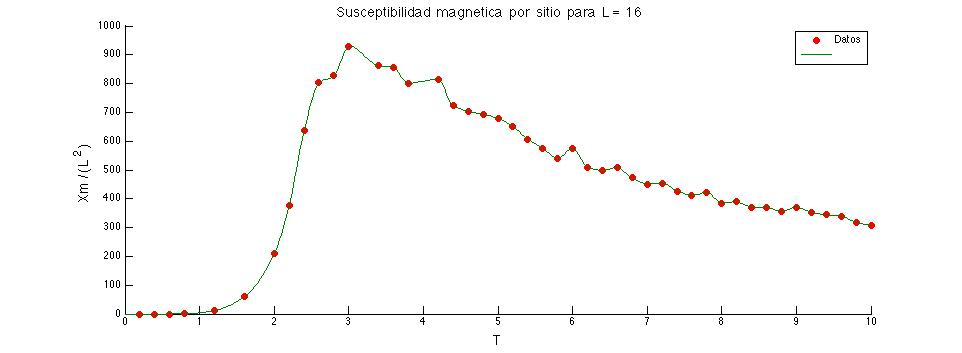
\includegraphics[height=8cm]{../graficos/Xm_L16.jpg}
\caption[width=5cm]{Susceptibilidad magn\'etica por sitio para $L$ = 16.}
\end{center}
\end{figure}

En los gr\'aficos se puede observar el aumento del $C_{v}$ y $\chi_{m}$ a medida que la temperatura se acerca al valor critico, donde las mismas son m\'aximas (cambio de fase). En este punto se puede ver la discontinuidad en $C_{v} = \frac{dE}{dT}$ y $\chi_{m} = \frac{dM}{d\beta}$, para luego decaer a valores cercanos a 0.

Para finalizar este ejercicio, se muestran los gr\'aficos obtenidos de $C_{v}$ y $\chi_{m}$ para $L$ = 32:

\begin{figure}[H]
\begin{center}
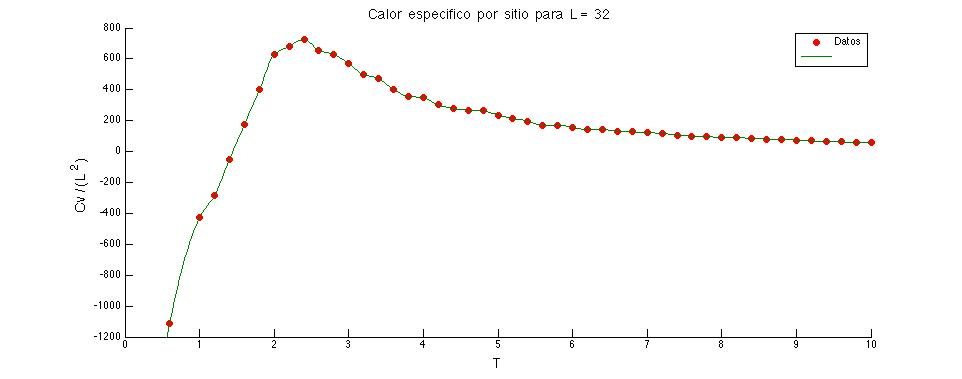
\includegraphics[height=8cm]{../graficos/Cv_L32.jpg}
\caption[width=5cm]{Calor espec\'ifico por sitio para $L$ = 32.}
\end{center}
\end{figure}

\begin{figure}[H]
\begin{center}
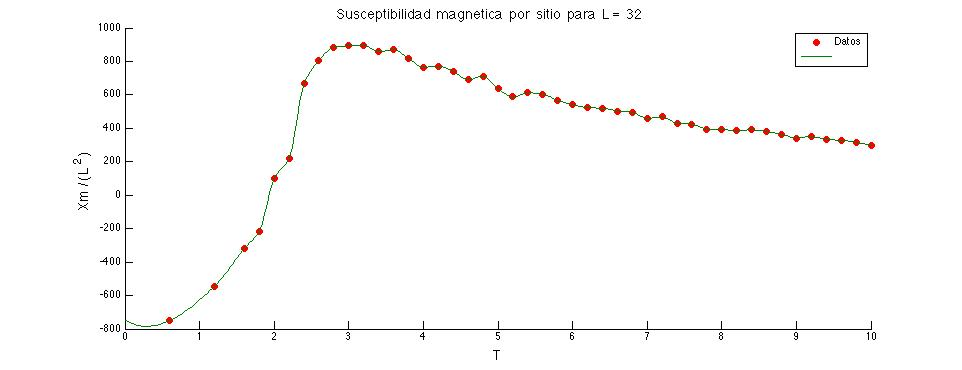
\includegraphics[height=8cm]{../graficos/Xm_L32.jpg}
\caption[width=5cm]{Susceptibilidad magn\'etica por sitio para $L$ = 32.}
\end{center}
\end{figure}

\subsection{Conclusiones}

Para $L$ = 32 se puede que el decaimiento de ambos observables es a\'un m\'as r\'apido con respecto a los correspondientes a $L$ = 16, luego de la temperatura cr\'itica $T_{c}$; concordando con mayor exactitud con el salto que produce la discontinuidad en las derivadas de $E$ y $M$.

En ambos casos, el cambio de fase observado en $C_{v}$ y $\chi_{m}$ se dio alrededor de un valor de la temperatura cr\'itica en $T_{c}$ = 2.27; de acuerdo con el mencionado en el enunciado para $T_{c} = \frac{2}{ln(1+\sqrt{2})} \approx 2.2691...$


\section{Ejercicio: Longitud de correlaci\'on en funci\'on de la temperatura}

Para calcular la longitud de correlaci\'on, se eligieron los vecinos a un spin cualquiera en cada iteraci\'on del c\'odigo; calculando primero la funci\'on de correlaci\'on entre ellos. 

A continuaci\'on se presentan los resultados para una red de tama\~no $L$ = 16 y $L$ = 32. La cantidad de iteraciones se mantuvo fija en $n$ = 3000, como en el ejercicio anterior:

\subsection{Resultados}

\begin{figure}[H]
\begin{center}
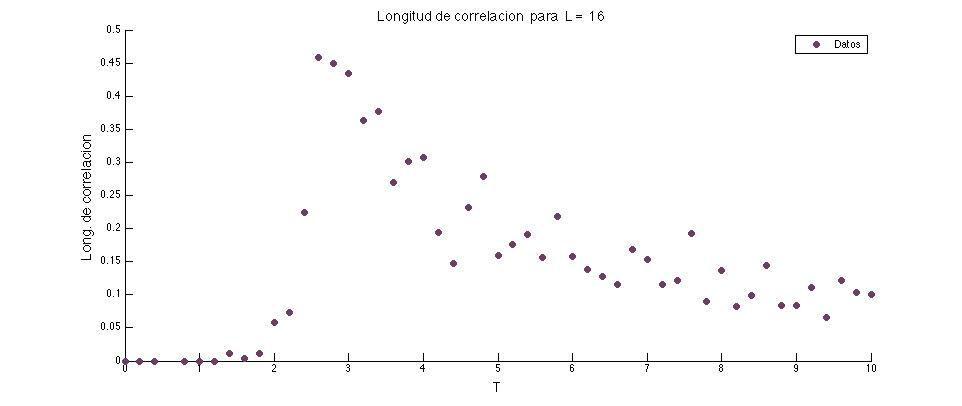
\includegraphics[height=8cm]{../graficos/Lcorr_L16.jpg}
\caption[width=5cm]{Longitud de correlaci\'on para $L$ = 36.}
\end{center}
\end{figure}

\begin{figure}[H]
\begin{center}
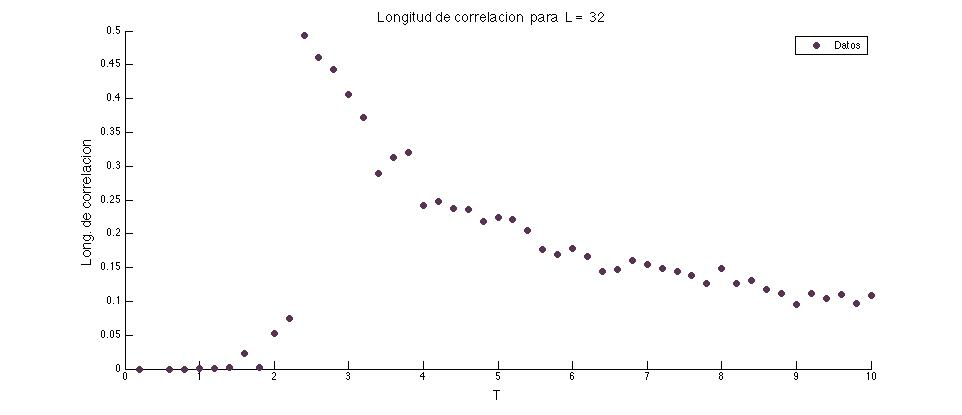
\includegraphics[height=8cm]{../graficos/Lcorr_L32.jpg}
\caption[width=5cm]{Longitud de correlaci\'on para $L$ = 32.}
\end{center}
\end{figure}

\subsection{Conclusiones}

En primer lugar, not\'e que los resultados tienen menor dispersi\'on para $L$ = 32, sobre todo para $T > T_{c}$; lo que permite inferir en primera instancia que a medida que $L$ aumenta, los valores se corresponden en mayor medida a la teor\'ia, la cual indica que en un entorno de $T_{c}$, la longitud de correlacion sigue una ley de potencias y no una exponencial como en el resto de las zonas.

Esto quiere decir que, a medida que la temperatura se acerca a $T_{c}$, la longitud de correlaci\'oon entre espines diverge, lo que implica que espines lejanos est\'an correlacionados, es decir, el estado de uno afecta a otro con una distancia mayor a la de sus primeros o segundos vecinos, por ejemplo. Por tanto, el sistema cerca de una transici\'on 
de fase pierde memoria de su estructura microsc\'opica y comienza a presentar nuevas correlaciones macrosc\'opicas de largo alcance.


\section{Ap\'endice}

\subsection{C\'odigo fuente de la funci\'on generadora de n\'umeros enteros aleatorios (/codigo/randint.m)}

\lstinputlisting[language=Matlab,breaklines]{../codigo/randint.m}

\subsection{C\'odigo fuente de la funci\'on de energ\'ia total del sistema (/codigo/En.m)}

\lstinputlisting[language=Matlab,breaklines]{../codigo/En.m}

\subsection{C\'odigo fuente de la funci\'on de Ising 2D en un paso (/codigo/ising2Dpaso.m)}

\lstinputlisting[language=Matlab,breaklines]{../codigo/ising2Dpaso.m}

\subsection{C\'odigo fuente de la funci\'on de Ising 2D para un valor de T (/codigo/ising2D0.m)}

\lstinputlisting[language=Matlab,breaklines]{../codigo/ising2D0.m}

\subsection{C\'odigo fuente de la funcion de Ising 2D para varios valores de T (/codigo/ising2D1.m)}

\lstinputlisting[language=Matlab,breaklines]{../codigo/ising2D1.m}

\end{document}
